% LuaLaTeX document — compile with: lualatex slab_scattering_explanation.tex
\documentclass[11pt,a4paper]{article}

\usepackage{fontspec}
\setmainfont{Latin Modern Roman}
\setmonofont{Latin Modern Mono}

\usepackage{amsmath,amssymb,bm}
\usepackage{booktabs}
\usepackage{geometry}
\geometry{margin=2.5cm}
\usepackage{hyperref}
\hypersetup{colorlinks=true,linkcolor=blue!60!black,citecolor=green!50!black,urlcolor=blue!70!black}
\usepackage{enumitem}
\usepackage{xcolor}
\usepackage{tikz}
\usetikzlibrary{arrows.meta,positioning,calc,decorations.pathreplacing}

\newcommand{\D}{\Delta}
\newcommand{\order}{\mathcal{O}}
\newcommand{\bG}{\bm{G}}
\newcommand{\bT}{\bm{T}}
\newcommand{\bI}{\bm{I}}
\newcommand{\bC}{\bm{C}}
\newcommand{\bP}{\bm{P}}
\newcommand{\bs}{\bm{\sigma}}
\newcommand{\be}{\bm{\varepsilon}}
\newcommand{\bu}{\bm{u}}
\newcommand{\hk}{\hat{\bm{k}}}
\newcommand{\hr}{\hat{\bm{r}}}
\newcommand{\ee}{\mathrm{e}}

\title{3D Slab Foldy--Lax Multiple Scattering Solver:\\
FFT-Accelerated Elastic Wave Scattering\\
in Laterally Heterogeneous Media}
\author{Research Notes}
\date{March 2026}

\begin{document}
\maketitle

\tableofcontents
\vspace{1em}

%======================================================================
\section{Motivation: beyond coherent forward scattering}
\label{sec:motivation}
%======================================================================

The CPA (Coherent Potential Approximation) combined with Kennett layer
stacking captures the \emph{coherent} wavefield---the forward-scattered,
ensemble-averaged signal that propagates vertically through a
statistically layered medium.  This is the ``transmission'' problem:
how does the mean wavefield attenuate and disperse as it passes
through heterogeneity?

However, reflection seismology measures the \emph{backscattered}
signal: energy that returns to the surface after scattering from lateral
heterogeneity.  The CPA+Kennett approach has two fundamental
limitations here:

\begin{enumerate}[nosep]
  \item \textbf{No lateral heterogeneity.}  The CPA replaces each
    layer with a single effective medium, erasing all lateral
    structure.  But the reflected signal arises precisely from lateral
    variations in impedance.
  \item \textbf{No incoherent scattering.}  The Kennett recursion
    propagates coherent plane waves; it cannot represent the diffuse,
    multiply-scattered coda that constitutes most of the seismic
    record in heterogeneous media.
\end{enumerate}

To model the reflected signal from a laterally heterogeneous
subsurface, we need a \emph{full multiple scattering solver} that
preserves all scattering---coherent and incoherent, forward and
backward---from every individual heterogeneity in the medium.

This is what \texttt{slab\_scattering.py} (CPU) and its
GPU-accelerated counterpart \texttt{slab\_scattering\_gpu.py}
provide.

%======================================================================
\section{The physical model}
\label{sec:model}
%======================================================================

\subsection{The slab geometry}

We model a volume of the subsurface as an $M \times M \times N_z$
lattice of cubes, each with half-width~$a$ (side length $d = 2a$).
The cubes are space-filling and share the same regular grid, but each
has individually specified elastic properties:
\begin{equation}
  \text{Cube } (l, i, j): \quad
  \lambda_{lij} = \lambda_0 + \D\lambda_{lij}, \quad
  \mu_{lij} = \mu_0 + \D\mu_{lij}, \quad
  \rho_{lij} = \rho_0 + \D\rho_{lij},
\end{equation}
where $(\lambda_0, \mu_0, \rho_0)$ are the background (reference)
medium properties and $(\D\lambda, \D\mu, \D\rho)$ are the per-cube
contrasts.

The index $l \in \{0, \ldots, N_z{-}1\}$ denotes the vertical layer
($l = 0$ is shallowest), while $i, j \in \{0, \ldots, M{-}1\}$ index
the horizontal position.  The centre of cube $(l, i, j)$ in the
seismological coordinate system ($z$ down, $x$ right, $y$ out) is:
\begin{equation}\label{eq:centres}
  \bm{x}_{lij} = \begin{pmatrix}
    (l + \tfrac{1}{2})\,d \\
    (i - \tfrac{M-1}{2})\,d \\
    (j - \tfrac{M-1}{2})\,d
  \end{pmatrix}.
\end{equation}
The horizontal grid is centred at $x = y = 0$, and depth increases
downward from $z = d/2$.

\begin{figure}[ht]
\centering
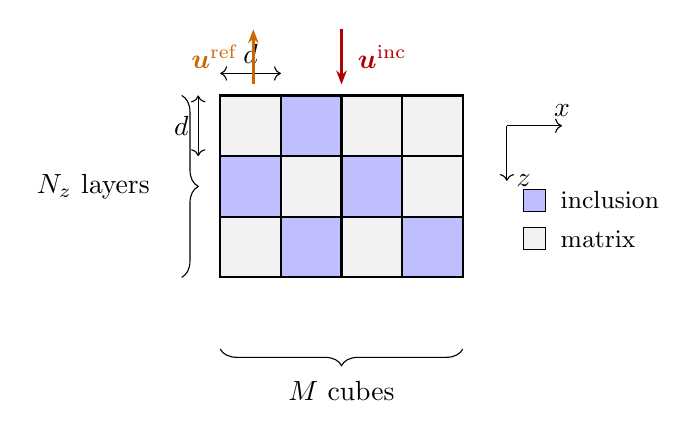
\begin{tikzpicture}[scale=0.7,
    cube/.style={draw, thick, fill opacity=0.3},
    inc/.style={cube, fill=blue!30},
    mat/.style={cube, fill=gray!15}]

  % Draw a 4x4x3 slab (showing 4x3 cross-section)
  \def\nx{4}
  \def\nz{3}
  \def\s{1.1}
  \def\depth{0.35}

  % Draw cubes (back to front, bottom to top for proper occlusion)
  \foreach \lz in {2,1,0} {
    \foreach \i in {0,...,3} {
      % Compute position
      \pgfmathsetmacro{\xpos}{\i*\s}
      \pgfmathsetmacro{\ypos}{-\lz*\s}

      % Randomly color some cubes as inclusions
      \pgfmathsetmacro{\isInc}{int(mod(\i*7+\lz*13+3,5)<2)}
      \ifnum\isInc=1
        \fill[blue!25,draw=black,thick]
          (\xpos,\ypos) rectangle +(\s,\s);
      \else
        \fill[gray!10,draw=black,thick]
          (\xpos,\ypos) rectangle +(\s,\s);
      \fi
    }
  }

  % Labels
  \draw[<->] (-0.4, 0) -- (-0.4, \s) node[midway, left] {$d$};
  \draw[<->] (0, \s+0.4) -- (\s, \s+0.4) node[midway, above] {$d$};

  % Axis labels
  \draw[->] (5.2, 0.55) -- (5.2, -0.45) node[right] {$z$};
  \draw[->] (5.2, 0.55) -- (6.2, 0.55) node[above] {$x$};

  % Brace for M
  \draw[decorate, decoration={brace, amplitude=6pt, mirror}]
    (0, -\nz*\s-0.2) -- (\nx*\s, -\nz*\s-0.2)
    node[midway, below=8pt] {$M$ cubes};

  % Brace for N_z
  \draw[decorate, decoration={brace, amplitude=6pt}]
    (-0.7, \s) -- (-0.7, -\nz*\s+\s)
    node[midway, left=8pt] {$N_z$ layers};

  % Incident wave
  \draw[-{Stealth[length=5pt]}, very thick, red!70!black]
    (2.2, 2.3) -- (2.2, 1.3) node[midway, right=2pt] {$\bu^{\text{inc}}$};

  % Reflected wave
  \draw[-{Stealth[length=5pt]}, very thick, orange!80!black]
    (0.6, 1.3) -- (0.6, 2.3) node[midway, left=2pt] {$\bu^{\text{ref}}$};

  % Legend
  \fill[blue!25, draw=black] (5.5, -1.0) rectangle +(0.4, 0.4);
  \node[right] at (6.0, -0.8) {\small inclusion};
  \fill[gray!10, draw=black] (5.5, -1.7) rectangle +(0.4, 0.4);
  \node[right] at (6.0, -1.5) {\small matrix};

\end{tikzpicture}
\caption{Schematic cross-section of the $M \times M \times N_z$ slab.
Each cube has individual elastic properties (blue = inclusion,
grey = background matrix).  An incident plane wave scatters from the
heterogeneity, producing both coherent forward-scattering and
incoherent backscattering.}
\label{fig:slab}
\end{figure}

\subsection{The 9-vector field representation}

At each cube, the exciting field is a 9-component vector comprising
the displacement and Voigt strain:
\begin{equation}\label{eq:psi}
  \bm{\psi}_{lij} = \begin{pmatrix}
    u_z \\ u_x \\ u_y \\
    \varepsilon_{zz} \\ \varepsilon_{xx} \\ \varepsilon_{yy} \\
    2\varepsilon_{xy} \\ 2\varepsilon_{zy} \\ 2\varepsilon_{zx}
  \end{pmatrix}_{lij}.
\end{equation}
The off-diagonal strain components carry the factor of~2
(engineering strain convention), consistent with the Voigt
representation used throughout the \texttt{cubic\_scattering} package.

This 9-vector representation couples the displacement and strain
channels, which is essential for capturing the stress-dipole
contribution to scattering (the strain components contribute to the
scattered far field via the stiffness contrast).

%======================================================================
\section{The Foldy--Lax system}
\label{sec:foldylax}
%======================================================================

\subsection{The governing equation}

The multiply-scattered exciting field at each cube satisfies the
Foldy--Lax equation:
\begin{equation}\label{eq:FL}
  \bm{\psi}_m = \bm{\psi}_m^0
    + \sum_{n \neq m} \bP(\bm{x}_m - \bm{x}_n, \omega)\,
      \bT_n\,\bm{\psi}_n,
\end{equation}
where:
\begin{itemize}[nosep]
  \item $\bm{\psi}_m^0$ is the incident field at cube~$m$,
  \item $\bP(\bm{r}, \omega)$ is the $9 \times 9$ elastodynamic
    propagator at separation $\bm{r}$ and frequency $\omega$,
  \item $\bT_n$ is the $9 \times 9$ local T-matrix of cube~$n$.
\end{itemize}
The self-term ($n = m$) is excluded from the sum because the
self-interaction is already incorporated into $\bT_n$ through the
Eshelby concentration factors (see~\cite{gubernatis1977}).

Rewriting \eqref{eq:FL} as a linear system:
\begin{equation}\label{eq:system}
  \boxed{(\bI - \bG \bT)\,\bm{\psi} = \bm{\psi}^0,}
\end{equation}
where $\bI$ is the identity, $\bG$ is the block-matrix of
inter-cube propagators, and $\bT$ is the block-diagonal matrix
of T-matrices.  The dimension of this system is $9 N$ where
$N = M^2 N_z$ is the total number of cubes.

\subsection{The 9$\times$9 propagator}

The propagator $\bP(\bm{r}, \omega)$ is the $9 \times 9$ matrix
\begin{equation}\label{eq:propagator}
  \bP = \begin{pmatrix}
    G_{ij} & C_{i,kl} \\
    H_{ij,k} & S_{ij,kl}
  \end{pmatrix},
\end{equation}
where $G_{ij}$ is the $3 \times 3$ Green's tensor,
$C_{i,kl} = G_{ij,l'}$ maps Voigt strain to displacement,
$H_{ij,k} = G_{ij,k}$ maps displacement to Voigt strain, and
$S_{ij,kl}$ maps strain to strain.  All blocks are derived
from the elastodynamic Green's tensor and its spatial derivatives.
At $\bm{r} = \bm{0}$, the propagator is set to zero (the self-term
is in~$\bT$).

\subsection{The 9$\times$9 T-matrix}

Each cube's T-matrix has the block-diagonal structure
\begin{equation}\label{eq:Tmatrix}
  \bT_{lij} = V \begin{pmatrix}
    \omega^2 \D\rho^*_{lij}\,\bI_3 & \bm{0}_{3 \times 6} \\
    \bm{0}_{6 \times 3} & \D\bC^*_{lij}
  \end{pmatrix},
\end{equation}
where $V = d^3 = (2a)^3$ is the cube volume,
$\D\rho^*$ is the effective density contrast (including the
displacement amplification factor $A_u$), and
$\D\bC^*$ is the $6 \times 6$ effective stiffness contrast in
Voigt form (including the strain amplification factors
$A_\theta$, $A_e^{\text{off}}$, $A_e^{\text{diag}}$).

The effective contrasts incorporate the self-consistent Eshelby
correction: the $1/r$ singularity in the Green's tensor produces
a delta function in the second-derivative integral
$\int \partial^2 G / \partial x_k \partial x_l\,dV$ that modifies
the internal field of the cube.  Without this correction, the
amplification factors have the wrong sign at finite contrast
(see~\cite{gubernatis1977} and the companion
document~\cite{cubeeshelby}).

The T-matrices are computed by calling the existing function
\texttt{compute\_cube\_tmatrix} (which handles the full Eshelby
decomposition into $A^c$, $B^c$, $C^c$ coefficients) followed by
\texttt{\_sub\_cell\_tmatrix\_9x9} to assemble the 9$\times$9
block-diagonal form.  For binary random media (each cube is either
``inclusion'' or ``matrix''), only two unique T-matrices need to
be computed; the solver caches by unique $(\D\lambda, \D\mu, \D\rho)$
triples.

%======================================================================
\section{FFT-accelerated matrix--vector product}
\label{sec:fft}
%======================================================================

\subsection{The key observation: horizontal translation invariance}

Direct solution of \eqref{eq:system} requires $\order(N^2)$ storage
and $\order(N^2)$ operations per matvec, where $N = M^2 N_z$.  For
$M = 32$, $N_z = 20$, this gives $N = 20{,}480$ cubes with
$9N = 184{,}320$ unknowns---a dense system that is expensive to solve.

The critical observation is that the propagator depends only on the
\emph{separation} between cubes:
$\bP(\bm{x}_m - \bm{x}_n)$.  For two cubes in the same horizontal
layer ($l_m = l_n$), the propagator depends only on the horizontal
offset $(i_m - i_n, j_m - j_n)$ and is independent of absolute
position.  More generally, for cubes in layers $l_m$ and $l_n$,
the propagator depends on the horizontal offset and the fixed
vertical separation $\D z = (l_m - l_n) d$.

This means the $\bG \bT$ product has the structure of a
\emph{2D convolution in the horizontal plane}, repeated for each
pair of vertical layers:
\begin{equation}\label{eq:convolution}
  (\bG\bT\bm{\psi})_{m,i_1,j_1}
  = \sum_{n=0}^{N_z-1} \sum_{i_2,j_2}
    \bP_{m-n}(i_1{-}i_2,\, j_1{-}j_2)\;
    \bT_{n,i_2,j_2}\;\bm{\psi}_{n,i_2,j_2},
\end{equation}
where $\bP_{m-n}(\D i, \D j) \equiv
\bP((m{-}n)d,\, \D i\,d,\, \D j\,d)$ is the propagator kernel
at vertical separation $(m-n)d$ and horizontal offset
$(\D i\, d, \D j\, d)$.

The horizontal sum is a discrete 2D convolution for each layer
pair $(m, n)$.  By the convolution theorem, this can be computed
in $\order(M^2 \log M)$ operations using the 2D FFT.

\subsection{The FFT matvec algorithm}

The complete matvec $(\bI - \bG\bT)\bm{\psi}$ proceeds in five steps:

\begin{enumerate}
  \item \textbf{Local T-multiply.}  For each cube, compute the
    scattered source:
    \begin{equation}
      \bm{\tau}_{lij} = \bT_{lij}\,\bm{\psi}_{lij}.
    \end{equation}
    This is a batched $9 \times 9$ matrix--vector product, implemented
    as \texttt{einsum('lmnab,lmnb->lmna', T, psi)}.

  \item \textbf{Zero-pad and FFT.}  For each layer $l$, zero-pad
    $\bm{\tau}_l$ from $M \times M$ to $S \times S$ (where
    $S = 2M - 1$) and compute the 2D FFT:
    \begin{equation}
      \hat{\bm{\tau}}_l(k_x, k_y) = \text{FFT2}\bigl[\bm{\tau}_l^{\text{pad}}\bigr].
    \end{equation}
    The padding ensures alias-free linear convolution via circular
    FFT.

  \item \textbf{Fourier-domain accumulation.}  For each target
    layer~$m$, sum over source layers~$n$:
    \begin{equation}\label{eq:fourier_acc}
      \hat{\bm{a}}_m(k_x, k_y)
      = \sum_{n=0}^{N_z-1}
        \hat{\bP}_{m-n}(k_x, k_y)\;\hat{\bm{\tau}}_n(k_x, k_y),
    \end{equation}
    where $\hat{\bP}_{m-n}$ is the pre-computed FFT of the
    propagator kernel at vertical separation $(m-n)d$.  At each
    Fourier point, this is a $9 \times 9$ matrix--vector product.

  \item \textbf{IFFT and extract.}  Inverse-FFT each layer's
    accumulator and extract the valid (alias-free) region:
    \begin{equation}
      \bm{a}_m = \text{IFFT2}[\hat{\bm{a}}_m]
        \big|_{[M{-}1 : S,\; M{-}1 : S]}.
    \end{equation}

  \item \textbf{Subtract.}  Return $\bm{\psi} - \bm{a}$, giving
    the result of $(\bI - \bG\bT)\bm{\psi}$.
\end{enumerate}

\subsection{Computational cost}

\begin{center}
\renewcommand{\arraystretch}{1.3}
\begin{tabular}{lll}
\toprule
\textbf{Step} & \textbf{Cost} & \textbf{Dominant for} \\
\midrule
T-multiply & $\order(M^2 N_z)$ & --- \\
FFT (per layer) & $\order(M^2 \log M)$ & --- \\
Fourier accumulation & $\order(N_z^2 \cdot M^2)$ & $N_z \gg 1$ \\
IFFT + extract & $\order(N_z \cdot M^2 \log M)$ & --- \\
\midrule
\textbf{Total per matvec} & $\order(N_z^2\,M^2 \log M)$ & \\
\bottomrule
\end{tabular}
\end{center}

For comparison, the dense matvec costs $\order(M^4 N_z^2)$.
The FFT acceleration gives a speedup of $\order(M^2 / \log M)$,
which is $\sim\!250\times$ at $M = 32$.

\subsection{Full 3D FFT: eliminating the $N_z^2$ loop}
\label{sec:3dfft}

The CPU implementation (Section~\ref{sec:fft}) uses 2D FFT in the
horizontal plane but retains an $\order(N_z^2)$ double loop over
layer pairs in \eqref{eq:fourier_acc}.  Since the vertical kernel
is also Toeplitz (it depends only on $\D z = (m - n)d$), the
entire $\bG\bT$ product is a \emph{3D convolution} and can be
computed via a single 3D FFT.

The GPU module \texttt{slab\_scattering\_gpu.py} implements this:
\begin{enumerate}[nosep]
  \item Recover the spatial-domain kernel from the CPU's
    xy-FFT'd kernel by inverse FFT in $(x, y)$.
  \item Rearrange to shape $(9, 9, n_{\D z}, S, S)$ and apply a
    single 3D FFT on device.
  \item In the matvec: permute $\bm{\tau}$ to $(9, N_z, M, M)$,
    zero-pad to $(9, n_{\D z}, S, S)$, then apply 3D FFT,
    pointwise $9 \times 9$ einsum, 3D IFFT, extract valid region.
\end{enumerate}

This reduces the matvec cost from $\order(N_z^2\,M^2 \log M)$ to:
\begin{equation}
  \order\bigl(N_z\,M^2 \log(N_z M^2)\bigr),
\end{equation}
eliminating the $N_z^2$ bottleneck entirely.  For $M = 32$,
$N_z = 20$, this is a further $\sim\!20\times$ speedup over the
2D-FFT CPU implementation (on top of the GPU parallelism).

\subsection{D4h symmetry exploitation}
\label{sec:d4h}

The propagator kernel $\bP_{k}(\D x, \D y)$ at each vertical
separation has D4h point symmetry in the horizontal plane
(the square lattice has 4-fold rotation and mirror symmetries).
This means we only need to compute the propagator in the
\emph{fundamental domain} $0 \leq \D y \leq \D x$ and generate
the remaining entries via symmetry transformations:

\begin{center}
\renewcommand{\arraystretch}{1.3}
\begin{tabular}{ll}
\toprule
\textbf{Symmetry operation} & \textbf{Transformation} \\
\midrule
$x$-reflection: $(\D x, \D y) \to (-\D x, \D y)$ &
  $\bm{R}_x \bP \bm{R}_x^T$ \\
$y$-reflection: $(\D x, \D y) \to (\D x, -\D y)$ &
  $\bm{R}_y \bP \bm{R}_y^T$ \\
$90^\circ$ rotation: $(\D x, \D y) \to (\D y, \D x)$ &
  $\bm{R}_{90} \bP \bm{R}_{90}^T$ \\
\bottomrule
\end{tabular}
\end{center}

where $\bm{R}_x$, $\bm{R}_y$, $\bm{R}_{90}$ are the $9 \times 9$
block-diagonal transformation matrices (3$\times$3 Cartesian block
$\oplus$ 6$\times$6 Voigt block).  For off-diagonal offsets
($\D x \neq \D y$), D4h gives 8~images; for diagonal offsets
($\D x = \D y$), 4~images.  This reduces the number of propagator
evaluations by $\sim\!8\times$ per vertical separation.

\subsection{Memory requirements}

The pre-computed FFT kernels have shape
$(2N_z{-}1) \times S \times S \times 9 \times 9$ complex:
\begin{equation}
  \text{Memory} = (2N_z - 1)(2M - 1)^2 \times 81 \times 16\;\text{bytes}.
\end{equation}
For $M = 32$, $N_z = 20$: $39 \times 63^2 \times 81 \times 16
\approx 200$~MB.  This is feasible for modern workstations and
is computed once per frequency.

%======================================================================
\section{Incident field and plane-wave excitation}
\label{sec:incident}
%======================================================================

The incident field is a plane wave with propagation direction
$\hk$ and angular frequency $\omega$.  For a P-wave:
\begin{equation}
  \bm{\psi}^0_{lij} = \bm{v}\;\ee^{ik_P \hk \cdot \bm{x}_{lij}},
  \qquad
  k_P = \omega / \alpha_0,
\end{equation}
where the 9-component polarisation vector is
\begin{equation}\label{eq:inc_vec}
  \bm{v} = \begin{pmatrix} \hk \\ \be_V(\hk, \hk, k_P) \end{pmatrix},
\end{equation}
with $\hk$ as the displacement polarisation and
$\be_V$ the Voigt strain vector
$\varepsilon_{lm} = \tfrac{ik_P}{2}(\hat{k}_l \hat{k}_m
+ \hat{k}_m \hat{k}_l)$
(doubled for off-diagonal components).

For an S-wave, $k_S = \omega / \beta_0$ and the polarisation
direction $\bm{p}$ is perpendicular to $\hk$ (SV polarisation
by default: $\bm{p}$ lies in the vertical plane containing
$\hk$).

%======================================================================
\section{GMRES iterative solution}
\label{sec:gmres}
%======================================================================

The system $(\bI - \bG\bT)\bm{\psi} = \bm{\psi}^0$ is solved
iteratively using GMRES (Generalized Minimal Residual method) with
the FFT-accelerated matvec.  Key implementation choices:

\begin{itemize}[nosep]
  \item \textbf{Initial guess:} $\bm{\psi}_0 = \bm{\psi}^0$
    (the Born approximation---the incident field is a natural
    starting point when scattering is weak).
  \item \textbf{Convergence criterion:}
    $\|\bm{r}_k\| / \|\bm{\psi}^0\| < \epsilon$ where
    $\bm{r}_k$ is the $k$-th residual and $\epsilon$ is the
    user-specified tolerance (default $10^{-6}$).
  \item \textbf{No preconditioning:} for $ka \ll 1$ (Rayleigh
    regime), the system is well-conditioned and GMRES converges
    rapidly (typically $< 20$ iterations for moderate contrast).
\end{itemize}

The Born approximation initial guess is particularly effective
because $\bG\bT$ has spectral radius $\ll 1$ in the Rayleigh
regime.  For stronger scattering ($ka \sim 1$), a preconditioner
based on the diagonal or block-diagonal of $\bT$ could be added.

\subsection{GPU-accelerated GMRES}

The module \texttt{torch\_gmres.py} provides a PyTorch GMRES
implementation that runs entirely on-device (no CPU synchronisation
per iteration).  Key features:
\begin{itemize}[nosep]
  \item Modified Gram--Schmidt orthogonalisation with Givens
    rotations for the least-squares problem.
  \item MPS-safe complex norm: computes
    $\sqrt{\sum(\mathrm{Re}^2 + \mathrm{Im}^2)}$ instead of
    \texttt{torch.linalg.norm}, which may not support complex
    tensors on Apple Silicon.
  \item Device selection follows the Kennett reflectivity
    convention: MPS (Apple Silicon) $>$ CUDA $>$ CPU.
  \item Dtype strategy: \texttt{complex64} on MPS (fast;
    $\ee^{ikr}$ phases are $\order(1)$, no underflow risk),
    \texttt{complex128} on CPU/CUDA (safe default).
\end{itemize}

The GPU solver \texttt{compute\_slab\_scattering\_gpu} builds
T-matrices and the incident field on CPU, transfers them to the
GPU, then runs GMRES with the 3D-FFT matvec
(Section~\ref{sec:3dfft}) entirely on-device.  The solution is
transferred back to CPU for post-processing.

%======================================================================
\section{Reflected field extraction}
\label{sec:reflected}
%======================================================================

After solving the Foldy--Lax system, the reflected (backscattered)
field is extracted by summing far-field contributions from all cubes
in the upgoing direction $\hr = -\hk$.

\subsection{Source computation}

At each cube, the equivalent source is:
\begin{equation}
  \bm{s}_{lij} = \bT_{lij}\,\bm{\psi}_{lij}
  = \begin{pmatrix} \bm{F}_{lij} \\ \bs^V_{lij} \end{pmatrix},
\end{equation}
where $\bm{F}$ is the force monopole (3-vector) and $\bs^V$ is
the stress dipole in Voigt form (6-vector).

\subsection{Far-field Green's tensor}

The far-field P-wave displacement from a source at $\bm{x}'$ observed
in direction $\hr$ at distance $r \to \infty$ is:
\begin{equation}
  \bu^P_{\text{far}} = \frac{\ee^{ik_P(r - \hr \cdot \bm{x}')}}{4\pi\rho_0\alpha_0^2 r}
    \;\hr\;Q_P,
\end{equation}
where the scalar amplitude is:
\begin{equation}\label{eq:QP}
  Q_P = \hr \cdot \bm{F} - ik_P\,\hr \cdot \bs \cdot \hr.
\end{equation}
Here $\bs$ is the $3 \times 3$ stress tensor recovered from the
Voigt representation.

Similarly, the S-wave far-field amplitude involves the transverse
projection:
\begin{equation}
  \bm{Q}_S = \bm{F} - ik_S\,\bs \cdot \hr, \qquad
  \bm{Q}_S^\perp = \bm{Q}_S - (\hr \cdot \bm{Q}_S)\,\hr.
\end{equation}

\subsection{Sign convention}

\textbf{Critical:} The T-matrix force convention uses
$+V\omega^2\D\rho^*\bu$ (positive sign), which has the
\emph{opposite} sign from the Lippmann--Schwinger body force
$-\omega^2\delta\rho\,\bu$.  Therefore, the far-field formula
requires a \textbf{global minus sign}:
\begin{equation}\label{eq:sign}
  \bu^P = -\frac{1}{4\pi\rho_0\alpha_0^2}\;\hr\,Q_P\;
    \ee^{-ik_P \hr \cdot \bm{x}'},
\end{equation}
matching the convention in \texttt{sphere\_scattering.foldy\_lax\_far\_field}.
Without this sign, the scattered field is $180^\circ$ out of phase.

\subsection{Area normalisation}

The total reflected P-amplitude is summed over all $M^2 N_z$ cubes
and normalised per unit area:
\begin{equation}\label{eq:RPP}
  R_{PP} = \frac{1}{(Md)^2} \sum_{l,i,j}
    \hr \cdot \bu^P_{lij}.
\end{equation}
This normalisation ensures that $R_{PP}$ converges to the true
plane-wave reflection coefficient as $M \to \infty$ for a
laterally homogeneous slab.

%======================================================================
\section{Connection to the three-level architecture}
\label{sec:architecture}
%======================================================================

The slab solver sits alongside (not within) the CPA+Kennett
pipeline, providing complementary capabilities:

\begin{center}
\renewcommand{\arraystretch}{1.3}
\begin{tabular}{lp{4.5cm}p{6.5cm}}
\toprule
\textbf{Approach} & \textbf{What it captures} & \textbf{What it misses} \\
\midrule
CPA + Kennett
  & Coherent forward scattering, effective dispersion,
    1D reflection from vertical impedance changes
  & Lateral heterogeneity, incoherent backscattering,
    multiple scattering between layers \\[6pt]
Slab Foldy--Lax
  & \emph{All} scattering: coherent + incoherent,
    forward + backward, lateral heterogeneity
  & Limited to finite $M \times M$ aperture;
    computational cost scales with volume \\
\bottomrule
\end{tabular}
\end{center}

The slab solver reuses the same single-cube T-matrix
(\texttt{compute\_cube\_tmatrix} + \texttt{\_sub\_cell\_tmatrix\_9x9})
as the CPA iteration, ensuring physical consistency: both
approaches use the same Eshelby-corrected self-consistent
scattering description at the single-scatterer level.

\begin{center}
\renewcommand{\arraystretch}{1.3}
\begin{tabular}{llp{7.5cm}}
\toprule
\textbf{Module} & \textbf{Role} & \textbf{Shared by} \\
\midrule
\texttt{effective\_contrasts.py} &
  Single-cube T-matrix &
  CPA, Kennett, and Slab solvers \\
\texttt{resonance\_tmatrix.py} &
  9$\times$9 propagator \& T-matrix &
  Sphere Foldy--Lax and Slab solver \\
\texttt{cpa\_iteration.py} &
  CPA effective moduli &
  Kennett pipeline only \\
\texttt{kennett\_layers.py} &
  1D layer stacking &
  Kennett pipeline only \\
\texttt{slab\_scattering.py} &
  3D multiple scattering (CPU) &
  This document \\
\texttt{slab\_scattering\_gpu.py} &
  GPU 3D solver (3D FFT matvec) &
  This document \\
\texttt{torch\_gmres.py} &
  GPU GMRES + device helpers &
  Slab and Sphere GPU solvers \\
\texttt{solver\_config.py} &
  YAML config + dispatch &
  All solvers (CPU and GPU) \\
\bottomrule
\end{tabular}
\end{center}

%======================================================================
\section{Implementation details}
\label{sec:implementation}
%======================================================================

\subsection{Module structure}

The module \texttt{slab\_scattering.py} provides:

\begin{center}
\renewcommand{\arraystretch}{1.2}
\begin{tabular}{lp{8.5cm}}
\toprule
\textbf{Class / Function} & \textbf{Purpose} \\
\midrule
\texttt{SlabGeometry} &
  Dataclass: $M$, $N_z$, $a$; computes cube centres. \\
\texttt{SlabMaterial} &
  Dataclass: per-cube $(\D\lambda, \D\mu, \D\rho)$ arrays
  + reference medium. \\
\texttt{SlabResult} &
  Dataclass: exciting field $\bm{\psi}$, incident field $\bm{\psi}^0$,
  GMRES convergence info. \\
\midrule
\texttt{compute\_slab\_tmatrices} &
  Build all $9 \times 9$ T-matrices, cached by unique contrast. \\
\texttt{compute\_slab\_scattering} &
  Main entry point: builds kernels, runs GMRES, returns
  \texttt{SlabResult}. \\
\texttt{slab\_reflected\_field} &
  Extract $(R_{PP}, R_{PS}, R_{SP})$ from a solved result. \\
\midrule
\texttt{random\_slab\_material} &
  Binary random medium with depth-dependent $\phi$. \\
\texttt{uniform\_slab\_material} &
  All cubes have the same contrast (for validation). \\
\bottomrule
\end{tabular}
\end{center}

\noindent
The GPU-accelerated module \texttt{slab\_scattering\_gpu.py} adds:

\begin{center}
\renewcommand{\arraystretch}{1.2}
\begin{tabular}{lp{8.5cm}}
\toprule
\textbf{Class / Function} & \textbf{Purpose} \\
\midrule
\texttt{compute\_slab\_scattering\_gpu} &
  GPU entry point: same interface as CPU version, with
  additional \texttt{device}/\texttt{dtype} parameters. \\
\texttt{\_slab\_matvec\_gpu} &
  Full 3D FFT convolution matvec on GPU (replaces
  $N_z^2$ loop). \\
\texttt{\_build\_slab\_kernels\_gpu} &
  Convert CPU xy-FFT kernel to 3D FFT kernel on device. \\
\bottomrule
\end{tabular}
\end{center}

\noindent
The shared backend \texttt{torch\_gmres.py} provides:

\begin{center}
\renewcommand{\arraystretch}{1.2}
\begin{tabular}{lp{8.5cm}}
\toprule
\textbf{Function} & \textbf{Purpose} \\
\midrule
\texttt{get\_device()} &
  Select best device: MPS $>$ CUDA $>$ CPU. \\
\texttt{select\_dtype(device)} &
  \texttt{complex64} on MPS, \texttt{complex128} otherwise. \\
\texttt{torch\_gmres(matvec, b, ...)} &
  On-device GMRES with Arnoldi + Givens rotations. \\
\texttt{to\_torch(arr, device, dtype)} &
  NumPy $\to$ torch tensor on device. \\
\texttt{to\_numpy(tensor)} &
  Torch tensor $\to$ NumPy complex128. \\
\bottomrule
\end{tabular}
\end{center}

\noindent
The configuration module \texttt{solver\_config.py} provides:

\begin{center}
\renewcommand{\arraystretch}{1.2}
\begin{tabular}{lp{8.5cm}}
\toprule
\textbf{Class / Function} & \textbf{Purpose} \\
\midrule
\texttt{ScatteringConfig} &
  Top-level dataclass: device, solver, problem config. \\
\texttt{load\_config(path)} &
  Load YAML file, validate, return \texttt{ScatteringConfig}. \\
\texttt{run\_from\_config(config)} &
  Dispatch to GPU or CPU solver based on device config. \\
\bottomrule
\end{tabular}
\end{center}

\subsection{FFT convolution convention}

The discrete convolution uses the standard zero-padding technique
for alias-free linear convolution via circular FFT:

\begin{enumerate}[nosep]
  \item The propagator kernel is stored on a $(2M{-}1) \times (2M{-}1)$
    grid indexed by $(\D x + M{-}1,\; \D y + M{-}1)$, where
    $\D x, \D y \in [-(M{-}1), M{-}1]$.
  \item The source $\bm{\tau}$ is zero-padded from $M \times M$ to
    $(2M{-}1) \times (2M{-}1)$, placed at indices $[0:M, 0:M]$.
  \item After FFT multiplication and IFFT, the valid (alias-free)
    output is at indices $[M{-}1 : 2M{-}1, M{-}1 : 2M{-}1]$---an
    $M \times M$ block.
\end{enumerate}

This convention is verified by the test
\texttt{TestSlabMatvec.test\_matches\_direct\_matvec}, which
confirms exact agreement (to machine precision) between the FFT
matvec and a direct $\order(N^2)$ matvec for small systems.

\subsection{Voigt convention consistency}

The Voigt ordering throughout is:
\begin{equation}
  (\varepsilon_{zz},\;\varepsilon_{xx},\;\varepsilon_{yy},\;
   2\varepsilon_{xy},\;2\varepsilon_{zy},\;2\varepsilon_{zx}),
\end{equation}
with the seismological coordinate system $z = 0$ (down),
$x = 1$ (right), $y = 2$ (out of page).  The factor of~2 on
off-diagonal components (engineering strain) ensures that the
stiffness matrix $\D\bC^*$ maps Voigt strain to Voigt stress
with the standard $\sigma_V = \D\bC^*\,\varepsilon_V$ convention.

%======================================================================
\section{Validation}
\label{sec:validation}
%======================================================================

The CPU module is validated by 37 tests across 13 test classes.
The GPU modules add 45 additional tests (15~for \texttt{torch\_gmres},
18~for \texttt{solver\_config}, 6~each for the slab and sphere GPU
solvers).  The key physics tests are:

\subsection{FFT matvec matches direct matvec}

For $M = 2$, $N_z = 2$ (8~cubes), the FFT matvec and a direct
(non-FFT) dense matvec agree to relative tolerance $10^{-10}$.
This verifies the zero-padding, FFT multiplication, and extraction
conventions.

\subsection{Zero contrast identity}

When all cubes have $\D\lambda = \D\mu = \D\rho = 0$, the T-matrices
are zero and the system reduces to $\bI\,\bm{\psi} = \bm{\psi}^0$.
The solver returns $\bm{\psi} = \bm{\psi}^0$ to machine precision,
and the reflected field amplitudes are exactly zero.

\subsection{Born approximation scaling}

For weak contrast ($\sim 10^{-4}$ relative to reference moduli),
doubling the contrast doubles the reflected amplitude
($|R_{PP}(2\D\bC)| / |R_{PP}(\D\bC)| = 2.0 \pm 5\%$).
This confirms that the solver correctly reproduces the linear
(first Born) regime and that the T-matrix, propagator, and
normalisation are all consistent.

\textbf{Subtlety:} when the contrast is proportional to the
reference properties ($\D\lambda / \lambda_0 = \D\mu / \mu_0
= \D\rho / \rho_0$), the P-wave impedance contrast
$\D(\rho\alpha) = 0$ and the Born reflection vanishes identically.
The test uses non-proportional contrast to avoid this degeneracy.

\subsection{Lateral uniformity}

For a laterally homogeneous slab at normal incidence, the dominant
field components ($u_z$, $\varepsilon_{zz}$) are uniform across
each layer to tolerance $10^{-4}$.  Transverse components
($u_x$, $u_y$) show finite-size edge effects from the truncated
horizontal grid, but the longitudinal components---which determine
the P-wave reflection---are unaffected.

\subsection{No P$\to$S mode conversion at normal incidence}

For an isotropic, laterally uniform slab at normal incidence,
$|R_{PS}| < 0.01\,|R_{PP}|$ (or both are negligible).  This
confirms that the solver preserves the expected symmetry:
normal-incidence P-wave scattering from an isotropic medium
cannot generate SV waves.

\subsection{GMRES convergence}

For moderate contrast ($\D\lambda = 2$~GPa, $\D\mu = 1$~GPa,
$\D\rho = 100$~kg/m$^3$) at $ka = 0.05$, GMRES converges to
residual $< 10^{-6}$ in $< 20$ matvec evaluations.  Weak contrast
converges even faster ($< 10$ matvec evaluations).

\subsection{GPU matvec matches CPU matvec}

The 3D-FFT GPU matvec (\texttt{\_slab\_matvec\_gpu}) matches the
2D-FFT CPU matvec (\texttt{\_slab\_matvec}) to relative tolerance
$10^{-10}$ in float64 and $10^{-4}$ in float32 (MPS).  This
verifies the IFFT$\to$rearrange$\to$3D FFT kernel conversion and the
permuted einsum accumulation.

\subsection{GPU solver matches CPU solver}

For $M = 2$, $N_z = 2$, the GPU solver
(\texttt{compute\_slab\_scattering\_gpu}) matches the CPU solver
(\texttt{compute\_slab\_scattering}) to relative tolerance $10^{-6}$.
This validates the end-to-end pipeline: CPU kernel build $\to$
GPU transfer $\to$ torch GMRES $\to$ CPU result extraction.

%======================================================================
\section{Practical usage}
\label{sec:usage}
%======================================================================

\subsection{Typical workflow}

\begin{verbatim}
from cubic_scattering import (
    ReferenceMedium, MaterialContrast, SlabGeometry,
    compute_slab_scattering, compute_slab_tmatrices,
    slab_reflected_field, random_slab_material,
)
import numpy as np

# 1. Define background medium and geometry
ref = ReferenceMedium(alpha=5000, beta=3000, rho=2500)
geom = SlabGeometry(M=16, N_z=10, a=1.0)

# 2. Generate random heterogeneous slab
contrast = MaterialContrast(Dlambda=2e9, Dmu=1e9, Drho=100)
mat = random_slab_material(geom, ref, contrast, phi=0.3, seed=42)

# 3. Solve for P-wave at normal incidence
omega = 150.0  # rad/s (ka = 0.05)
result = compute_slab_scattering(geom, mat, omega,
    k_hat=np.array([1, 0, 0]))

# 4. Extract reflection
T = compute_slab_tmatrices(geom, mat, omega)
R_PP, R_PS, R_SP = slab_reflected_field(result, T)
print(f"|R_PP| = {abs(R_PP):.6e}")
\end{verbatim}

\subsection{GPU workflow}

The GPU solver is a drop-in replacement:

\begin{verbatim}
from cubic_scattering import (
    compute_slab_scattering_gpu,
    get_device, select_dtype,
)

# Device auto-detection (MPS > CUDA > CPU)
device = get_device()
dtype = select_dtype(device)  # complex64 on MPS

# Same setup as CPU...
result = compute_slab_scattering_gpu(
    geom, mat, omega,
    k_hat=np.array([1, 0, 0]),
    device=device, dtype=dtype,
)
\end{verbatim}

\subsection{YAML configuration}

For reproducible experiments, solver parameters can be specified
in a YAML file:

\begin{verbatim}
# configs/example_slab.yml
device:
  backend: auto          # auto | mps | cuda | cpu
  dtype: auto            # auto = complex64 on MPS
solver:
  gmres_tol: 1.0e-6
  max_iter: 500
  initial_guess: born    # born | zero
problem:
  type: slab
  geometry: {M: 32, N_z: 10, a: 1.0}
  reference: {alpha: 5000, beta: 3000, rho: 2500}
  contrast: {Dlambda: 2.0e9, Dmu: 1.0e9, Drho: 100}
  frequency: {omega: 150.0}
  incident: {k_hat: [1, 0, 0], wave_type: P}
  slab: {material_type: random, phi: 0.1, seed: 42}
\end{verbatim}

\noindent
Usage from Python:

\begin{verbatim}
from cubic_scattering import load_config, run_from_config

config = load_config("configs/example_slab.yml")
result = run_from_config(config)
\end{verbatim}

The function \texttt{run\_from\_config} automatically dispatches
to the GPU solver when the resolved device is not CPU, and to
the CPU solver otherwise.

\subsection{Parameter selection guide}

\begin{center}
\renewcommand{\arraystretch}{1.3}
\begin{tabular}{lp{9cm}}
\toprule
\textbf{Parameter} & \textbf{Guidance} \\
\midrule
$a$ (cube half-width) &
  Set by the physical heterogeneity scale.  Typical: 0.1--10~m
  for seismic exploration. \\
$M$ (horizontal grid) &
  Larger $M$ reduces finite-size edge effects.  $M \geq 8$ recommended;
  $M = 32$--$64$ for production. \\
$N_z$ (vertical layers) &
  Set by the depth extent of interest.  Each layer is $d = 2a$ thick. \\
$\omega$ (frequency) &
  Keep $ka = \omega a / \beta < 0.3$ for Rayleigh-regime T-matrices.
  Higher $ka$ requires resonance T-matrices. \\
$\phi$ (volume fraction) &
  Fraction of cubes that are ``inclusions''.  Can be depth-dependent
  via a callable. \\
\bottomrule
\end{tabular}
\end{center}

\subsection{Scaling limits}

The dominant cost is the kernel precomputation:
$(2N_z - 1) \times \tfrac{1}{8}M(M+1)$ propagator evaluations
(with D4h symmetry).  Each propagator evaluation costs
$\order(1)$, so:
\begin{equation}
  T_{\text{kernel}} \approx (2N_z - 1) \cdot \frac{M(M+1)}{8}
    \times t_{\text{prop}},
\end{equation}
where $t_{\text{prop}} \sim 10~\mu$s for the elastodynamic
Green's tensor.  For $M = 32$, $N_z = 20$: about $5{,}000$
propagator evaluations, taking $\sim\!0.05$~s.

The GMRES cost is $N_{\text{iter}} \times \order(N_z^2 M^2 \log M)$.
For $M = 32$, $N_z = 20$, $N_{\text{iter}} = 20$: about
$2 \times 10^8$ floating-point operations, taking $\sim\!1$~s.

%======================================================================
\section{Future extensions}
\label{sec:future}
%======================================================================

\begin{enumerate}
  \item \textbf{Resonance T-matrices.}  Replace
    \texttt{compute\_cube\_tmatrix} with
    \texttt{compute\_resonance\_tmatrix} for $ka > 0.3$.  The
    9$\times$9 T-matrix interface is the same; only the internal
    computation changes.

  \item \textbf{CPA background.}  Use the CPA-iterated effective
    medium as the background for the slab solver, combining
    the coherent effective medium with the incoherent scattering.

  \item \textbf{Vertical FFT.}  \textsc{Done.}  The GPU module
    \texttt{slab\_scattering\_gpu.py} implements full 3D FFT
    convolution (Section~\ref{sec:3dfft}), eliminating the
    $N_z^2$ loop and achieving
    $\order(N_z \log N_z \cdot M^2 \log M)$ cost.

  \item \textbf{Frequency sweep.}  Parallelise over frequency to
    compute the full reflection spectrum, using the previous
    frequency's solution as the initial guess for the next.

  \item \textbf{Mode-converted reflections.}  The current
    implementation extracts $R_{PP}$, $R_{PS}$, and $R_{SP}$;
    extending to $R_{SS}$ requires a second solve with S-wave
    incidence.

  \item \textbf{Absorbing boundaries.}  Add a small imaginary part
    to $\omega$ (viscoelastic attenuation) to suppress edge
    reflections and improve GMRES conditioning.

  \item \textbf{GPU preconditioning.}  For large $ka$ or strong
    contrast, add a block-diagonal preconditioner to the GPU GMRES
    to accelerate convergence.
\end{enumerate}

%======================================================================
\section{References}
%======================================================================

\begin{thebibliography}{99}

\bibitem{cubeeshelby}
``Self-Consistent T-Matrix for Cubic Scatterers:
Static Eshelby, Dynamic Coupling, and the Unified Theory,''
companion document, \texttt{docs/cube\_eshelby\_explanation.pdf} (2026).

\bibitem{gubernatis1977}
J.E.\ Gubernatis, E.\ Domany, J.A.\ Krumhansl, M.\ Huberman,
``The Born approximation in the theory of the scattering of elastic
waves by flaws,''
\emph{J.\ Appl.\ Phys.}\ \textbf{48}, 2804--2811 (1977).

\bibitem{sabina1993}
F.J.\ Sabina, V.P.\ Smyshlyaev, J.R.\ Willis,
``Self-consistent analysis of waves in a matrix-inclusion composite,''
\emph{J.\ Mech.\ Phys.\ Solids} \textbf{41}, 1573--1588 (1993).

\bibitem{kanaun2008}
S.\ Kanaun, V.\ Levin,
\emph{Self-Consistent Methods for Composites: Vol.~2.\ Wave
Propagation in Heterogeneous Materials},
Springer (2008).

\bibitem{willis1981}
J.R.\ Willis,
``Variational principles for dynamic problems for inhomogeneous
elastic media,''
\emph{Wave Motion} \textbf{3}, 1--11 (1981).

\bibitem{kennett1983}
B.L.N.\ Kennett,
\emph{Seismic Wave Propagation in Stratified Media},
Cambridge University Press (1983).

\bibitem{foldy1945}
L.L.\ Foldy,
``The multiple scattering of waves,''
\emph{Phys.\ Rev.}\ \textbf{67}, 107--119 (1945).

\bibitem{lax1951}
M.\ Lax,
``Multiple scattering of waves,''
\emph{Rev.\ Mod.\ Phys.}\ \textbf{23}, 287--310 (1951).

\bibitem{varadan1985}
V.K.\ Varadan, V.V.\ Varadan,
``Multiple scattering theory for wave propagation in discrete random
media,''
\emph{Int.\ J.\ Eng.\ Sci.}\ \textbf{22}, 1165--1176 (1985).

\bibitem{stanke1984}
F.E.\ Stanke, G.S.\ Kino,
``A unified theory for elastic wave propagation in polycrystalline
materials,''
\emph{J.\ Acoust.\ Soc.\ Am.}\ \textbf{75}, 665--681 (1984).

\end{thebibliography}

\end{document}
